%!TEX root = ../../main.tex
\section{Projektgennemførelse}
\subsection{Specificering af projektet}
Der var blevet lavet et opslag om at lave et kasse apparat til Katrines Kælder på Ingeniørhøjskolem i Århus. Her var der beskrevet krav til produktet og givet en beskrivelse af hvad de forventede. \newline
Hertil blev der opstillet nogle Use Cases så der kommer en helt klar afgrænsning om hvad produkt skal være i stand til når det er færdigt.\newline
For at give en bedre afgrænsning af krav til produktet er der blevet brugt MoSCoW-metoden. Ved hjælp af denne er der blevet sat nogle funtionelle og ikke-funtionelle krav. 

\subsection{V-Modellen}

V-Modellen, som er en udviklingsmodel, er blevet brugt i dette projekt til at lave test løbende. Da der laves test sideløbende sikres der at systemet virker efter hensigten. På figur \ref{VModel} kan V-Modellen ses.

\begin{figure}[H]
	\centering
	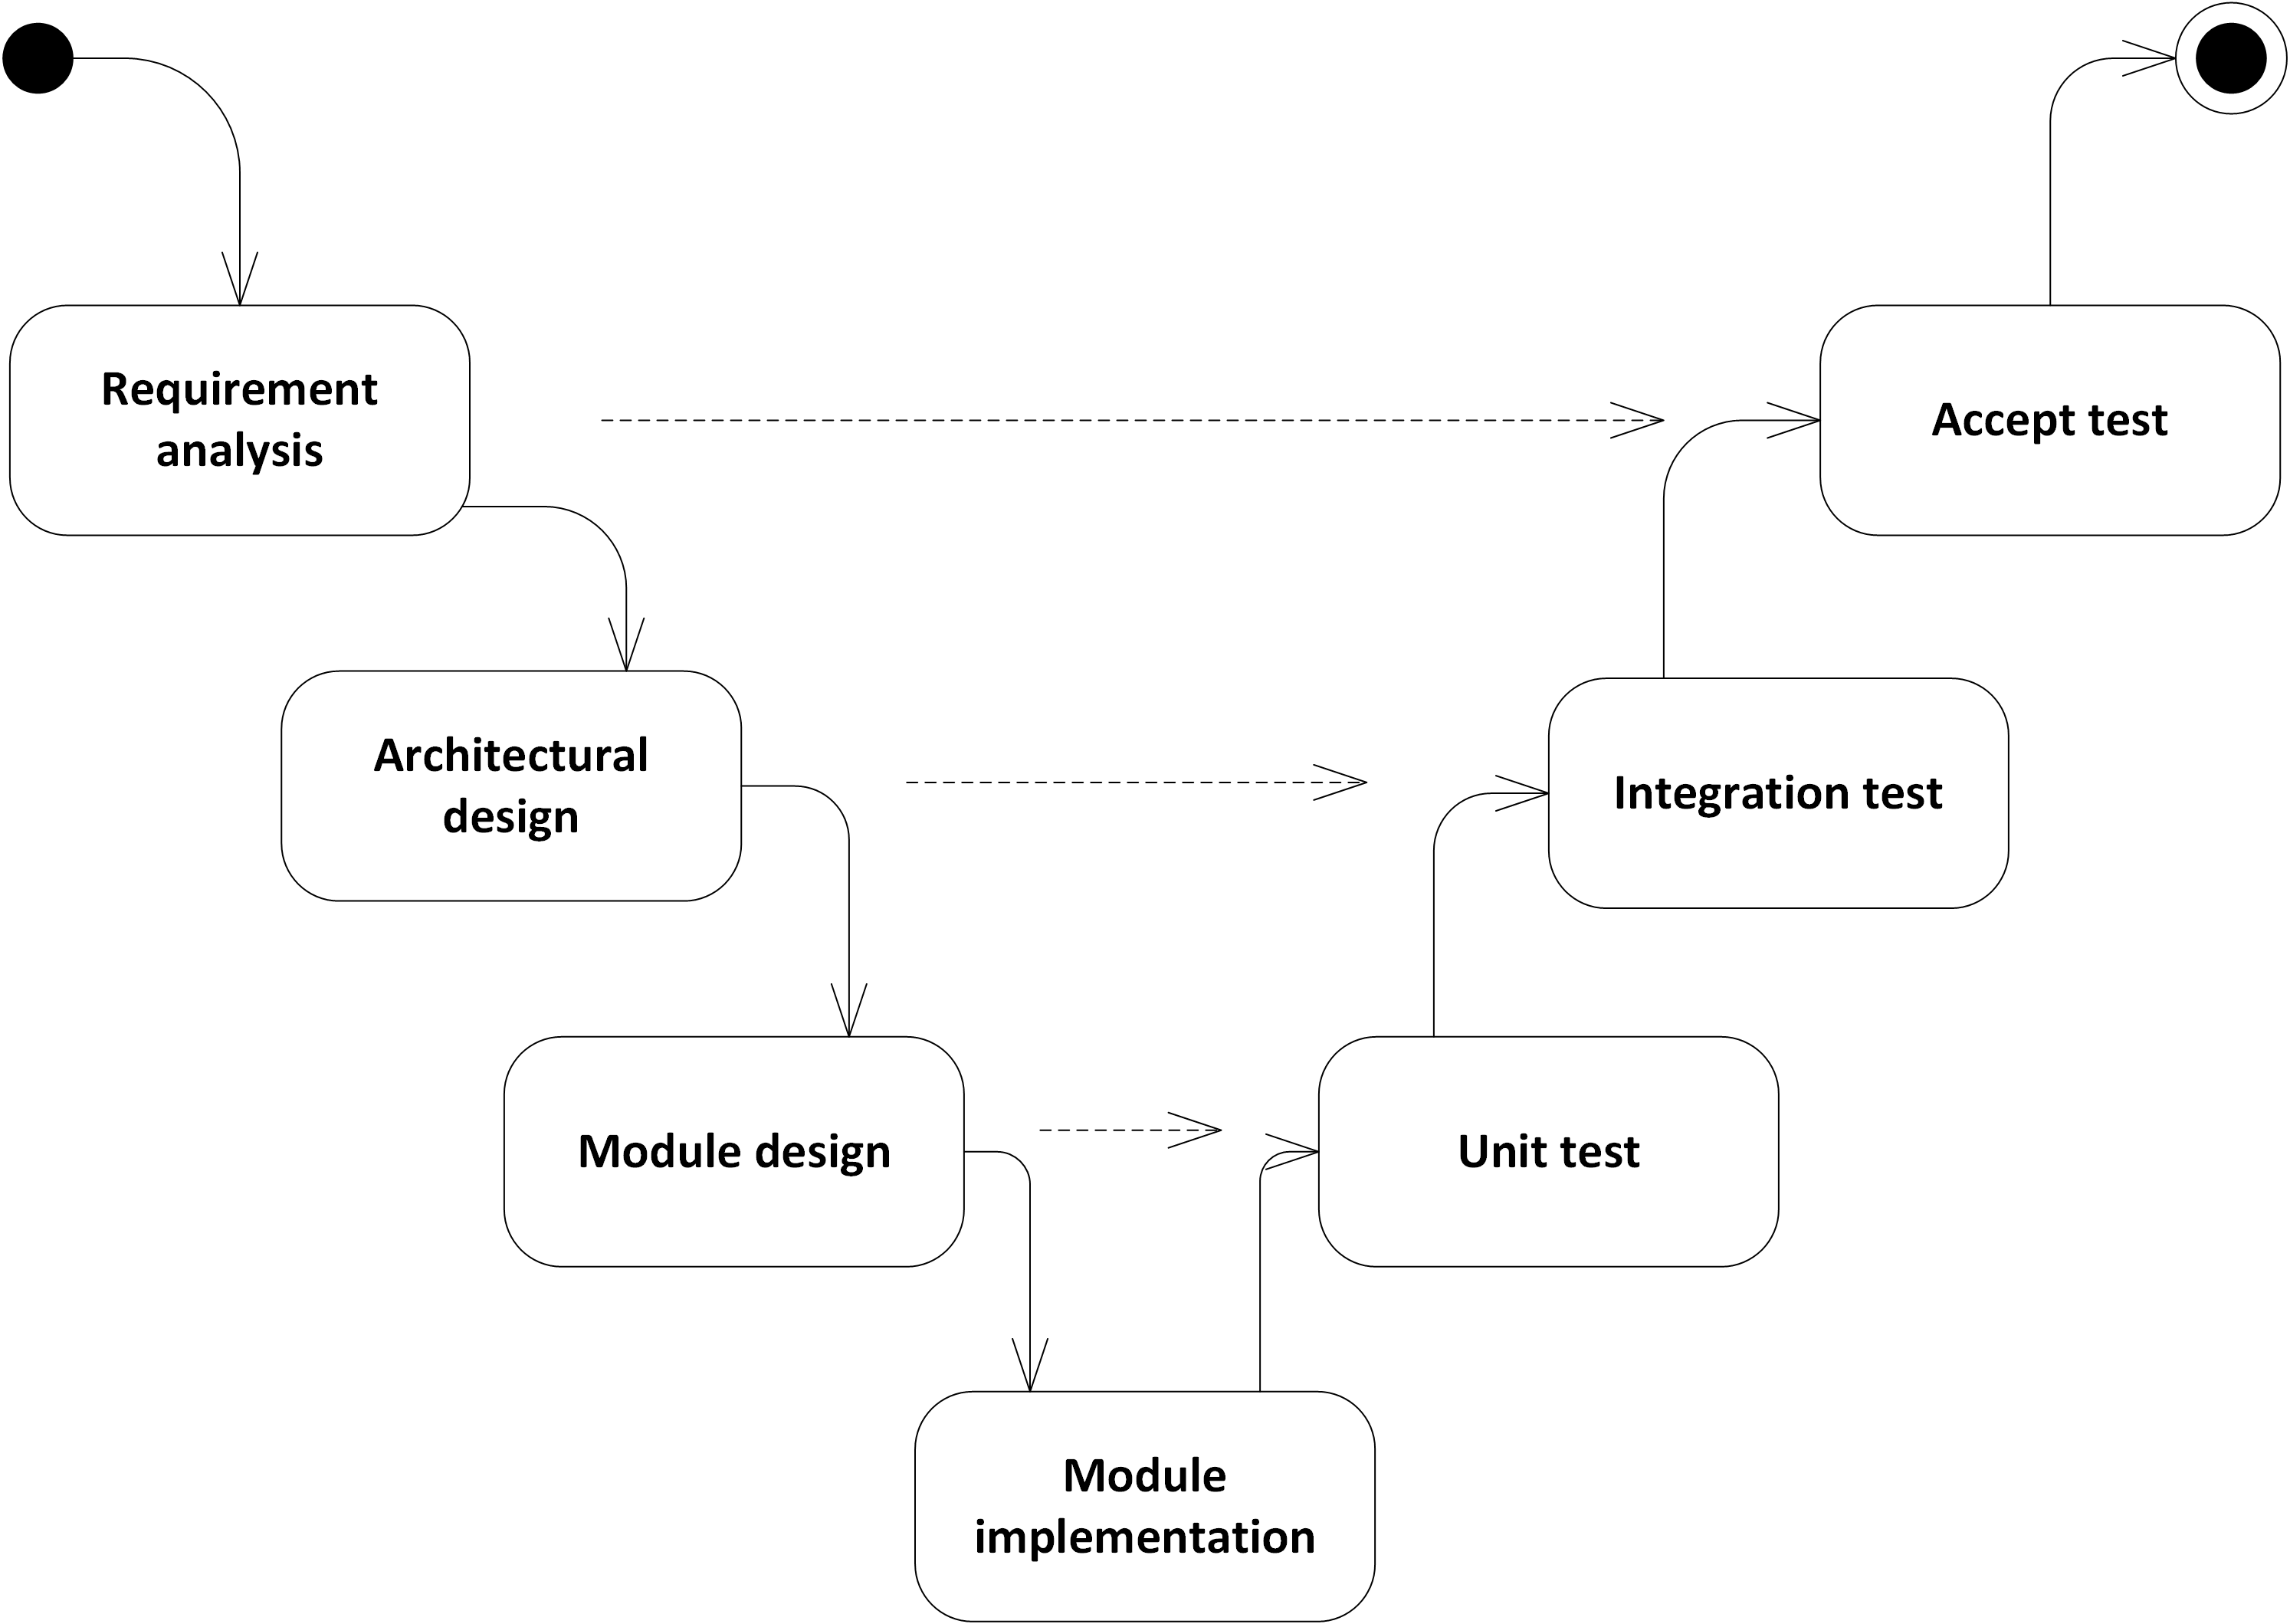
\includegraphics[scale=1.0]{Rapport/VModel.PNG}
	\caption{V-Modellen}
	\label{VModel}
\end{figure} 


\subsection{Arbejdsmetode}
Arbejdet med projektet er gjort rent iterativt og med SCRUM som dominerende proces, i den forstand at der er blevet arbejdet i sprint af to uger ad gangen. I disse sprint er der blevet fastlagt nogle arbejdsopgaver som skulle udføres. Til dette er er det ikke sådan at større dele af projektet er blevet lavet færdige før man gik videre. Alle dele af projektet er blevet lavet i små dele, hvor de har kunne spille sammen til en vis forstand så der hele tiden har været en smule sammenhold i projektet. 

\subsection{Proces}
Processen i dette semester projekt har været agil og, som nævnt tidligere, med SCRUM som dominerende proces.\newline
Der er de fleste dage blevet afholdt et dagligt SCRUM møde hvor der er blevet talt om hvilke arbejdsopgaver der er blevet udført og hvilke der mangler. I starten af semesteret blev daily SCRUM udført ca. hver anden dag, mens der senere på semestret blev afholdt et møde hver dag. \newline
Da den ene i projektgruppen er medarbejder hos kunden af produktet, har der hele tiden været en form for kontakt til kunden så der kunne ses hvis projektet var på vej ud på et vildspor eller om det der blev lavet var på sin plads. 


